\section{Impresiones}

\begin{center}
	\begin{tabular}{p{8cm} p{8cm}}
        \texttt{a = [(1, 2), (3, 4), (5, 6)]} \newline \texttt{print(len(a))}& \texttt{a = [[1], [2]]} \newline \texttt{a.append([3, 4, 5])} \newline \texttt{print(len(a))} \\
        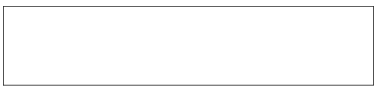
\includegraphics[scale=0.8]{Imagenes/rectangulo} & 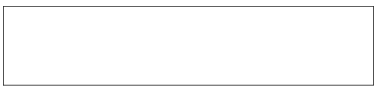
\includegraphics[scale=0.8]{Imagenes/rectangulo}\\
        \texttt{d = \{'a':'b','b':'c','c':'a'\}} \newline \texttt{a = ['d','e','a']} \newline \texttt{for c in d:} \newline \texttt{\-\ \-\ if c in a:} \newline \texttt{\-\ \-\ \-\ \-\ print(d[c])} & \texttt{t = [(25, (1, 9)), (15, (2, 11))]} \newline \texttt{s = 0}   \newline \texttt{for i in t:}  \newline \texttt{\-\ \-\ a, b = i}  \newline \texttt{\-\ \-\ c, d = b}  \newline \texttt{\-\ \-\ s += c} \newline \texttt{print(s)}\\
        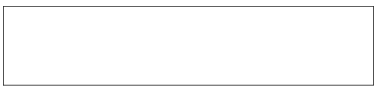
\includegraphics[scale=0.8]{Imagenes/rectangulo} & 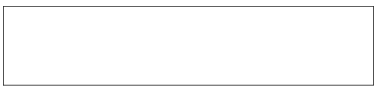
\includegraphics[scale=0.8]{Imagenes/rectangulo}\\
        \texttt{def f(x):} \newline \texttt{\-\ \-\ x = 18} \newline \texttt{\-\ \-\ return x} \newline \texttt{x = 10} \newline \texttt{print(f(f(f(x))))} & \texttt{def f(a, b):}\newline \texttt{\-\ \-\ return a * b}\newline \texttt{def g(a, b):}\newline \texttt{\-\ \-\ return f(b, a + b)}\newline \texttt{a, b = (2, 1)}\newline \texttt{print(f(g(b, a), g(a, b)))} \\
        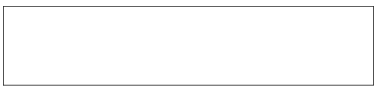
\includegraphics[scale=0.8]{Imagenes/rectangulo} & 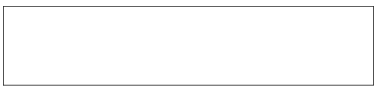
\includegraphics[scale=0.8]{Imagenes/rectangulo}
    \end{tabular}
\end{center}

